% !TEX program = lualatex
\documentclass[aspectratio=43,professionalfonts,handout]{beamer}
\usepackage{beamer_template}

\newcommand{\LectureNum}{7}
\newcommand{\LectureTitle}{対数関数}
\newcommand{\TextPages}{p.\,115-118}
\newcommand{\NextTopic}{常用対数}
\newcommand{\NextPages}{p.\,118-121}
\newcommand{\CourseName}{基礎数学B}
\renewcommand{\TermName}{後期}

\begin{document}

% -----------------------------------------------
% スライド1: 表紙＋目標＋用語・定義
% -----------------------------------------------
\begin{frame}{\CourseName\quad 第\LectureNum 回「\LectureTitle 」}
  {\small \TermName\quad \TeacherName\quad ／\quad 教科書 \TextPages\quad
  \textbf{目標}：対数関数 y=logₐx のグラフと性質を理解し、方程式・不等式を解ける}

  \begin{block}{用語・定義}
  \begin{description}[labelwidth=5.5em]
    \item[\kw{対数関数：y=logₐx}] ~
    \item[\kw{単調増加（a>1）・単調減少（0<a<1）}] ~
    \item[\kw{漸近線：x=0（y軸）}] ~
    \item[\kw{真数条件の重要性}] ~
  \end{description}
  \end{block}
\end{frame}

% -----------------------------------------------
% スライド2: 公式・性質
% -----------------------------------------------
\begin{frame}{公式・性質}
  \begin{block}{}
  \begin{itemize}
    \item 点(1,0)を必ず通る
    \item a>1：右上がり、0<a<1：右下がり
    \item 対数方程式：真数をまとめて指数に戻す
  \end{itemize}
  \end{block}
\end{frame}

% -----------------------------------------------
% スライド3: 図・グラフ（TikZコードを手動追加）
% -----------------------------------------------
\begin{frame}{図・グラフ}
  \centering
  % TODO: y=log₂x と y=log₁/₂x の比較（y軸対称）
  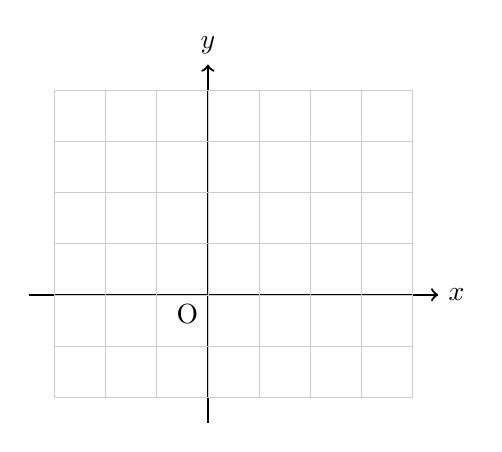
\begin{tikzpicture}[scale=0.65]
    \draw[->,thick] (-3.5,0) -- (4.5,0) node[right]{$x$};
    \draw[->,thick] (0,-2.5) -- (0,4.5) node[above]{$y$};
    \node[below left] at (0,0) {O};
    \draw[gray!40, very thin] (-3,-2) grid (4,4);
    % ここにグラフを描画
  \end{tikzpicture}
\end{frame}

% -----------------------------------------------
% スライド4: 例1→問1
% -----------------------------------------------
\begin{frame}{例1→問1}
  \begin{exampleblock}{例1) p.118（グラフをかけ・値域）}
    （板書で解説）
  \end{exampleblock}

  \vfill

  \begin{block}{問1) p.118\quad 自分で解いてみよう}
    （ノートに解くこと）
  \end{block}
\end{frame}

% -----------------------------------------------
% スライド5: 例2→問2
% -----------------------------------------------
\begin{frame}{例2→問2}
  \begin{exampleblock}{例題2) p.120（対数方程式・不等式）}
    （板書で解説）
  \end{exampleblock}

  \vfill

  \begin{block}{問2) p.120\quad 自分で解いてみよう}
    （ノートに解くこと）
  \end{block}
\end{frame}

% -----------------------------------------------
% まとめ
% -----------------------------------------------
\begin{frame}{まとめ}
  \begin{itemize}
    \item % TODO: まとめを記入
  \end{itemize}

  \vfill
  {\small 基本問題：232, 233, 234, 235, 236}
\end{frame}

\end{document}
